\documentclass[11pt, a4paper, english]{amsart}
\usepackage{amsmath} % utilities for mathematics
\usepackage{amsthm} % utilities for theorem environment
\usepackage{amssymb} % loads mathematical fonts
\usepackage[dvipsnames]{xcolor}
\usepackage{amscd} % utilities for commutative diagrams
\usepackage{mathtools}

\usepackage{subcaption}% <-- added

\usepackage{array} % core package
\usepackage{newtxtext,newtxmath} %fuente

\usepackage[cal=boondoxo,scr=euler]{mathalfa}
\usepackage[backref=page,linktocpage]{hyperref} % permits navigating on the pdf
\usepackage{cleveref} % smart referencing
\usepackage{caption} %
\usepackage{graphics,graphicx} % permits putting images
\usepackage{tikz,tikz-cd} % tool for diagrams

%\usetikzlibrary{graphdrawing.force}% quotes library is for the [""] edges
\usetikzlibrary{graphs,graphs.standard,calc}

\usetikzlibrary{decorations.pathreplacing,}%angles,quotes

\usepackage{enumerate} % permits enumerating using letters or other symbols

\DeclareMathAlphabet{\mathsf}{OT1}{\sfdefault}{m}{n}

\newcommand{\nocontentsline}[3]{}
\newcommand{\tocless}[2]{\bgroup\let\addcontentsline=\nocontentsline#1{#2}\egroup}


\usepackage[margin=1.25in]{geometry}
%\usepackage[textwidth=360pt,textheight=615pt]{geometry}
\linespread{1.08}
%\setlength\parindent{0.3in}

\usepackage{verbatim}


\usepackage{scalerel}

\makeatletter
\def\dual#1{\expandafter\dual@aux#1\@nil}
\def\dual@aux#1/#2\@nil{\begin{tabular}{@{}c@{}}#1\\#2\end{tabular}}
\makeatother

\makeatletter
\@namedef{subjclassname@2020}{\textup{2020} Mathematics Subject Classification}
\makeatother


\newcommand{\stirlingtwo}[2]{\biggl\{\genfrac{}{}{0pt}{}{#1}{#2}\biggr\}}
\newcommand{\tstirlingtwo}[2]{\left\{\genfrac{}{}{0pt}{}{#1}{#2}\right\}}
%\renewcommand{\tilde}{\widetilde}
%\renewcommand{\widetilde}{\wwtilde}

\DeclareMathAlphabet{\amathbb}{U}{bbold}{m}{n}


\newcommand{\mfrak}[1]{\scaleobj{0.93}{\mathfrak{#1}}}

\hypersetup{
    colorlinks = true,
    linkbordercolor = {white},
    linkcolor = {BrickRed},
    anchorcolor = {black},
    citecolor = {BrickRed},
    filecolor = {cyan},
    menucolor = {BrickRed},
    runcolor = {cyan},
    urlcolor = {black}
}

\usetikzlibrary{automata}
\usepackage{bbm}

\newtheoremstyle{teoremas}% <name>
{11pt}% <Space above>
{11pt}% <Space below>
{\itshape}% <Body font>
{}% <Indent amount>
{\bfseries}% <Theorem head font>
{}% <Punctuation after theorem head>
{.5em}% <Space after theorem headi>
{}% <Theorem head spec (can be left empty, meaning `normal')>



\theoremstyle{teoremas}
\newtheorem{theorem}{Theorem}[section]
\newtheorem{corollary}[theorem]{Corollary}
\newtheorem{lemma}[theorem]{Lemma}
\newtheorem{proposition}[theorem]{Proposition}

\newtheoremstyle{definition}% <name>
{11pt}% <Space above>
{11pt}% <Space below>
{}% <Body font>
{}% <Indent amount>
{\bfseries}% <Theorem head font>
{}% <Punctuation after theorem head>
{.5em}% <Space after theorem headi>
{}% <Theorem head spec (can be left empty, meaning `normal')>

\theoremstyle{definition}
\newtheorem{definition}[theorem]{Definition}
\newtheorem{thmdefinition}[theorem]{Theorem-Definition}

\newtheorem{conjecture}[theorem]{Conjecture}
\newtheorem{openproblem}[theorem]{Open Problem}
\newtheorem{problem}[theorem]{Problem}
\newtheorem{question}[theorem]{Question}
\newtheorem{example}[theorem]{Example}
\newtheorem{remark}[theorem]{Remark}

\crefname{theorem}{theorem}{theorems}
\Crefname{theorem}{Theorem}{Theorems}
\crefname{lemma}{lemma}{lemmas}
\Crefname{lemma}{Lemma}{Lemmas}
\crefname{proposition}{proposition}{propositions}
\Crefname{proposition}{Proposition}{Propositions}

\DeclareMathOperator{\rk}{rk}
\DeclareMathOperator{\cusp}{cusp}
\DeclareMathOperator{\Rel}{Rel}
\DeclareMathOperator{\Poin}{Poin}
\DeclareMathOperator{\Tor}{Tor}
\DeclareMathOperator{\Ext}{Ext}

\newcommand{\M}{\mathsf{M}}
%\newcommand{\B}{\mathsf{B}} let us only write \U_{n,n} for boolean matroids
\newcommand{\N}{\mathsf{N}}
\newcommand{\U}{\mathsf{U}}
\newcommand{\cI}{\mathcal{I}}
\newcommand{\A}{\mathrm{A}}
\newcommand{\Q}{\mathbb{Q}}
\newcommand{\R}{\mathbb{R}}
\newcommand{\Z}{\mathbb{Z}}
\newcommand{\LL}{\mathsf{\Lambda}}
\newcommand{\PP}{\mathsf{\Pi}}
\newcommand{\C}{\mathsf{C}}
\renewcommand{\lambda}{\uplambda}

\newcommand{\Hilb}{\operatorname{Hilb}}
\newcommand{\rank}{\operatorname{rk}}
\newcommand{\corank}{\operatorname{crk}}
\newcommand{\cl}{\operatorname{cl}}
\renewcommand{\H}{\mathrm{H}}
\newcommand{\CH}{\mathrm{CH}}
\newcommand{\aug}{\operatorname{aug}}
\newcommand{\IH}{\mathrm{IH}}
\newcommand{\uH}{\underline{\mathrm{H}}}
\newcommand{\uCH}{\underline{\mathrm{CH}}}
\newcommand\size[1]{|#1|}
\DeclareMathOperator{\Pal}{\mathrm{Pal}}
\DeclareMathOperator{\Poly}{\mathrm{Poly}}

\newcommand{\cL}{\mathcal{L}}
\newcommand{\cH}{\mathcal{H}}
\newcommand{\Rep}{\operatorname{Rep}}
\newcommand{\gr}{\operatorname{gr}}
\newcommand{\VRep}{\operatorname{VRep}}
\newcommand{\Ind}{\operatorname{Ind}}
\newcommand{\Res}{\operatorname{Res}}
\newcommand{\Aut}{\operatorname{Aut}}
\newcommand{\col}{\operatorname{col}}
\newcommand{\asc}{\operatorname{asc}}
\newcommand{\bad}{\operatorname{bad}}
\newcommand{\des}{\operatorname{des}}
\newcommand{\luis}{\textcolor{NavyBlue}}
\newcommand{\qbinom}[2]{\begin{bmatrix} #1 \\ #2 \end{bmatrix}_q}



\newcommand\rev[1]{#1^{\operatorname{rev}}}

\AtBeginDocument{%
   \def\MR#1{}
}


%% preliminary version only
\begin{comment}
 \usepackage{prelim2e}
 \renewcommand{\PrelimText}{\sf\scriptsize --- INCOMPLETE DRAFT of \today ---}
 \marginparwidth=0.75in
 \usepackage[notcite,notref]{showkeys}
 \usepackage[colorinlistoftodos,bordercolor=orange,backgroundcolor=orange!20,linecolor=orange,textsize=scriptsize]{todonotes}

 \usepackage{prelim2e}
 \usepackage[us,24hr]{datetime}
 \renewcommand{\PrelimText}{\sf\scriptsize ---\,Version of \today \,-\,\currenttime\,---}
\end{comment}



\title{Inverse Kazhdan--Lusztig polynomials\\ of matroids under deletion}

\author[T.~Braden]
{Tom~Braden}

\address{(T.~Braden)
University of Massachusetts Amherst, Amherst, MA, USA
}
\email{braden@umass.edu}


\author[L.~Ferroni]{Luis~Ferroni}

\address{(L.~Ferroni)
  Institute for Advanced Study, Princeton, NJ, USA
}
\email{ferroni@ias.edu}

\thanks{Luis Ferroni is a member at the Institute for Advanced Study, supported by the Minerva Research Foundation, and was also partially supported by the Swedish Research Council, Grant 2018-03968. Jacob Matherne and Nutan Nepal were supported by NSF Grant DMS-2452179 and Simons Foundation Travel Support for Mathematicians Award MPS-TSM00007970.}



\author[J.~P.~Matherne]{Jacob~P.~Matherne}

\address{(J. P. Matherne)
Department of Mathematics, North Carolina State University, Raleigh, NC, USA.
}
\email{jpmather@ncsu.edu}

\author[N.~Nepal]{Nutan Nepal}

\address{(N. Nepal)
Department of Mathematics, North Carolina State University, Raleigh, NC, USA.
}
\email{nnepal2@ncsu.edu}

\subjclass[2020]{Primary: 05B35}

\allowdisplaybreaks

\begin{document}

\begin{abstract}
    We give a ``deletion formula" for the inverse Kazhdan--Lusztig polynomial of a matroid: it relates the inverse Kazhdan--Lusztig polynomial of a matroid to that of a single non-coloop element deletion, and it is analogous to the deletion formula of Braden--Vysogorets for Kazhdan--Lusztig polynomials.  As an application of our deletion formula, we produce a counterexample to a recent conjecture of Xie and Zhang concerning the real-rootedness of the Hadamard product of the inverse Kazhdan--Lusztig polynomial with a binomial.  \textcolor{Bittersweet}{Furthermore, we ...}
\end{abstract}

\maketitle

\section{Introduction}

The Kazhdan--Lusztig polynomial $P_{\M}(t)$ is a fundamental invariant associated with any matroid $\M$. It was introduced by Elias, Proudfoot, and Wakefield in \cite{EPW16}. This polynomial, denoted $P_{\M}(t)$, exhibits formal similarities to the Kazhdan--Lusztig polynomials defined for Bruhat intervals of Coxeter groups. The coefficients of $P_{\M}(t)$ depend only on the lattice of flats $\mathcal{L}(\M)$ of the matroid and, in fact, they can be expressed as signed integer combinations of the flag Whitney numbers counting chains of flats with specified ranks (see \cite{proudfoot-xu-young}).

The Kazhdan--Lusztig polynomial of $\M$ plays a significant role in the \emph{singular} Hodge theory of matroids developed by Braden, Huh, Matherne, Proudfoot, and Wang in \cite{braden-huh-matherne-proudfoot-wang}. Two further polynomial invariants that are often studied in this context are the \emph{inverse Kazhdan--Lusztig polynomial of a matroid}, introduced by Gao and Xie \cite{gao-xie} and denoted $Q_{\M}(x)$, and the $Z$-polynomial introduced by Proudfoot, Xu, and Young \cite{proudfoot-xu-young}, and denoted $Z_{\M}(x)$. One of the main contributions in \cite{braden-huh-matherne-proudfoot-wang} consists of interpreting these three polynomials in the following way:
\begin{itemize}
    \item $P_{\M}(x)$ is the Hilbert series of the stalk of the intersection cohomology module of $\M$ at the empty set.
    \item $Z_{\M}(x)$ is the Hilbert series of the intersection cohomology module of $\M$.
    \item $Q_{\M}(x)$ is the Hilbert series of the trivial graded module in the Rouquier complex of $\M$.
\end{itemize}

The three interpretations above imply that these three polynomials appearing have nonnegative coefficients for every matroid $\M$. However, computing the above polynomials is often a daunting task even for small matroids.

In \cite{braden-vysogorets}, Braden and Vysogorets presented a formula that relates the Kazhdan--Lusztig polynomial
of a matroid $\M$ to that of the matroid obtained by deleting an element $i$, denoted $\M\setminus i$, as well as various restrictions and contractions of $\M$. Specifically, for a simple matroid $\M$ where $i$ is not a coloop, their main result states:

\begin{theorem}[{\cite[Theorem~2.8]{braden-vysogorets}}]
    Let $\M$ be a loopless matroid of rank $k$, and let $i\in E$ be an element of the ground set that is not a coloop. Then,
    \begin{align*}
        P_{\M}(x) & = P_{\M\smallsetminus\{i\}}(x) - xP_{\M/\{i\}}(x) + \sum_{F\in\mathscr{S}_i} \tau\left(\M/{(F\cup\{i\})}\right)\, x^{\frac{k - \rk(F)}{2}}\, P_{\M|_F}(x), \\
        Z_{\M}(x) & = Z_{\M\smallsetminus\{i\}}(x) + \sum_{F\in\mathscr{S}_i} \tau\left(\M/{(F\cup\{i\})}\right)\, x^{\frac{k - \rk(F)}{2}}\, Z_{\M|_F}(x).
    \end{align*}
\end{theorem}

In the above statement, the notation $\underline{\mathscr{S}}_i$ stands for a distinguished set of flats:
\begin{equation}\label{eq:S_i}
    \underline{\mathscr{S}}_i = \underline{\mathscr{S}}_i(\M) = \left\{ F \in \mathcal{L}(\M): \varnothing \subsetneq F\subsetneq E\smallsetminus\{i\} \text{ and } F\cup\{i\}\in \mathcal{L}(\M)\right\},
\end{equation}
whereas $\tau(\M)$ denotes
\[ \tau(\M) :=
    \begin{cases}
        [x^{\frac{\rk(\M)-1}{2}}] P_{\M}(x) & \text{if $\rk(\M)$ is odd,}  \\
        0                                   & \text{if $\rk(\M)$ is even.}
    \end{cases}
\]

\textcolor{red}{Luis: We should introduce and expand about the relevance of $Y_{\M}(x)$ (see below). }



\subsection{Main results}

Let us introduce a counterpart for the sets $\underline{\mathscr{S}}_i$ appearing in equation~\eqref{eq:S_i}. We define
\begin{equation}\label{eq:T_i}
    \mathscr{T}_i := \left\{ F \in \mathcal{L}(\M): i\in F \text{ and } F\setminus\{i\}\notin \mathcal{L}(\M)\right\}.
\end{equation}


\begin{theorem}\label{thm:deletion_formula_Q}
    Let $\M$ be a matroid on $E$ and let $i\in E$ be an element that is not a coloop. Then, the following identity holds:
    \[ Q_{\M}(x) = Q_{\M\smallsetminus i}(x) + (1+x) Q_{\M/i}(x) - \sum_{F\in \mathcal{T}_i} \tau(\M|_F/i)\, x^{\rk(F)/2}\, Q_{\M/F}(x).\]
\end{theorem}

We now introduce the $Y$-polynomial of a matroid $\M$, which is defined as:
\begin{equation}\label{eq:Y_polynomial}
    Y_{\M}(x) := (-1)^{\rk(\M)}\sum_{F\in \mathcal{L}(\M)} (-1)^{\rk(F)} x^{\rk(\M) - \rk(F)} \mu[F,E] Q_{\M|_F}(x),
\end{equation}
where $\mu[F,E]$ is the Möbius function of the interval $[F,E]$ in the lattice of flats $\mathcal{L}(\M)$.

\begin{theorem}
    Let $\M$ be a matroid on $E$ and let $i\in E$ be an element that is not a coloop. Then, the following identity holds:
    \[ Y_{\M}(x) = Y_{\M\smallsetminus i}(x) + (1+x) Y_{\M/i}(x) - \sum_{F\in \mathcal{T}_i} \tau(\M|_F/i)\, x^{\rk(F)/2}\, Y_{\M/F}(x).\]
\end{theorem}

\begin{remark}
    The deletion formulas for $Q_{\M}(x)$ and $Y_{\M}(x)$ look exactly the same. Compare this against the deletion formulas of $P_{\M}(x)$ and $Z_{\M}(x)$.
\end{remark}



\begin{corollary}
    Let $\mathsf{C}_{a,b}$ be the graphic matroid that results from gluing two cycles of length $a$ and $b$ along an edge. Then,
    \begin{multline*} Q_{\mathsf{C}_{a,b}}(x) = Q_{\U_{n-2,n-1}}(x)  + (1+x) Q_{\U_{a-2,a-1}}(x)\, Q_{\U_{b-2,b-1}}(x) \\- \left(\tau(\U_{a-2,a-1})\, x^{\frac{a-1}{2}}\, Q_{\U_{b-2,b-1}}(x) + \tau(\U_{b-2,b-1})\, x^{\frac{b-1}{2}} \,Q_{\U_{a-2,a-1}}(x)\right).
    \end{multline*}
    where $n = a+b-1$.
\end{corollary}

\begin{example}
    In Figure~\ref{fig:two-cycles} we depicted the graph that induces the graphic matroid $\mathsf{C}_{4,6}$.
    \begin{figure}[ht]
        \centering
        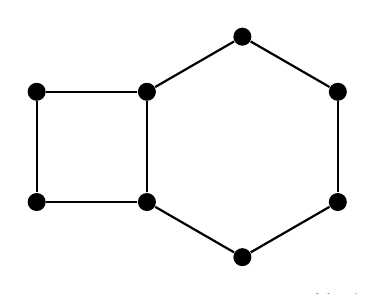
\begin{tikzpicture}
            [scale=0.7,auto=center,every node/.style={circle, fill=black, inner sep=2.3pt},every edge/.append style = {thick}]
            \tikzstyle{edges} = [thick];
            \node (a1) at (0,0) {};
            \node (a2) at (0,2)  {};
            \node (a3) at (1.7320,3)  {};
            \node (a4) at (2*1.7320,2) {};
            \node (a5) at (2*1.7320,0)  {};
            \node (a6) at (2*1.7320/2,-1)  {};
            \node (a7) at (-2,2) {};
            \node (a8) at (-2,0) {};
            \draw[edges] (a1) -- (a2);
            \draw[edges] (a2) -- (a3);
            \draw[edges] (a3) -- (a4);
            \draw[edges] (a4) -- (a5);
            \draw[edges] (a5) -- (a6);
            \draw[edges] (a6) -- (a1);
            \draw[edges] (a1) -- (a8);
            \draw[edges] (a2) -- (a7);
            \draw[edges] (a7) -- (a8);
        \end{tikzpicture} \caption{The graphic matroid $\mathsf{C}_{4,6}$.}\label{fig:two-cycles}
    \end{figure}
\end{example}

\begin{theorem}
    Let $\M$ be a corank $2$ matroid without coloops. Assume that for each $r$, $\lambda_r$ denotes the number of stressed subsets of rank $r$ and size $r+1$ in $\M$. Then
    \begin{align*}
        Q_{\M}(x) & = Q_{\U_{n-2,n}}(x) - \sum_{r} \lambda_{r} \sum_{a=2}^{n-r-1} \left(Q_{\C_{a,n+1-a}}(x) - Q_{\U_{a-1,a}}(x)\, Q_{\U_{n-a-1,n-a}}(x)\right), \\
        Y_{\M}(x) & = Y_{\U_{n-2,n}}(x) - \sum_{r} \lambda_{r} \sum_{a=2}^{n-r-1} \left(Y_{\C_{a,n+1-a}}(x) - Y_{\U_{a-1,a}}(x)\, Y_{\U_{n-a-1,n-a}}(x)\right).
    \end{align*}
    In particular, if $\M$ arises from a partition $\lambda$ of $[n]$, then
    \begin{align*}
        Q_{\M}(x) & = Q_{\U_{n-2,n}}(x) - \sum_{\substack{S\in \lambda \\ |S|\geq 2}} \sum_{a=2}^{|S|} \left(Q_{\C_{a,n+1-a}}(x) - Q_{\U_{a-1,a}}(x)\, Q_{\U_{n-a-1,n-a}}(x)\right),\\
        Y_{\M}(x) & = Y_{\U_{n-2,n}}(x) - \sum_{\substack{S\in \lambda \\ |S|\geq 2}}\sum_{a=2}^{|S|} \left(Y_{\C_{a,n+1-a}}(x) - Y_{\U_{a-1,a}}(x)\, Y_{\U_{n-a-1,n-a}}(x)\right).
    \end{align*}
\end{theorem}



\begin{theorem}
    There is a counterexample to Conjecture ? which consists of a matroid of rank $19$ on $21$ elements.
\end{theorem}


\section{Proof of the deletion formulas}

Let $\M$ be a matroid and $\cL(\M)$ be its lattice of flats. Following \cite{braden-vysogorets}, we define the module $\cH(\M)$ of $\M$ as the free $\mathbb{Z}[x, x^{-1}]$-module generated by the elements of $\cL(\M)$.
Elements of $\cH(\M)$ are formal sums of the form
\[
    \alpha = \sum_{F \in \cL(\M)} \alpha_F \cdot F, \quad \alpha_F \in \mathbb{Z}
    [x, x^{-1}].
\]
The module $\cH(\M)$ admits the Kazhdan--Lusztig basis $\zeta^F$ for $F \in \cL(\M)$ defined by
\[
    \zeta^F = \sum_{G \leq F} x^{\rk(F) - \rk(G)} P_{\M_G^F}(x^{-2}) \cdot G.
\]
where $P_{\M_G^F}(x)$ is the Kazhdan--Lusztig polynomial of the matroid $\M_G^F$.

Let $\hat{Q}_\M(x)$ denote the inverse of the Kazhdan--Lusztig polynomial, $P_\M(x)$, of $\M$ with respect to the incidence algebra of $\cL(\M)$. Then, we have
\begin{equation}
    Q_\M(x) = (-1)^{\rk(\M)} \hat{Q}_\M(x).
\end{equation}

\begin{lemma}\label{lem:standard_basis_in_zeta}
    The standard basis $\{F\}_{F \in \cL(\M)}$ of $\cH(\M)$ satisfies
    \begin{equation}
        \label{cob-lemma}
        F = \sum_{G \leq F} t^{\rk(F) - \rk(G)} \hat{Q}_{\M_G^F}(t^{-2}) \cdot \zeta^G.
    \end{equation}
\end{lemma}

\subsection{Homomorphism \text{$\Delta: \cH(\M) \to \cH(\M\setminus i)$}}\label{sec:delta}

Let $i$ be an element of the ground set of $\M$ that is not a coloop.
There is a surjective map $\cL(\M) \to \cL(\M\setminus i)$ sending a flat $F \in \cL(\M)$ to $F\setminus i \in \cL(\M\setminus i)$.
There also exists a module homomorphism $\Delta: \cH(\M) \to \cH(\M\setminus i)$ which
is $\mathbb{Z}[x, x^{-1}]$-linear and is defined on the basis elements $F \in \cL(\M)$ by
$\Delta(F) = x^{\rk_{\M\setminus i}(F\setminus i)- \rk_\M(F)} \cdot (F\setminus i)$. In particular, we have
\begin{equation}
    \Delta(F) = \begin{cases}
        F                          & \text{if }F\not\ni i                                      \\
        F\setminus i               & \text{if } F\ni i \text{ and }F\setminus i \notin \cL(\M) \\
        x^{-1}\cdot (F\setminus i) & \text{if } F\ni i \text{ and }F\setminus i \in \cL(\M).
    \end{cases}
\end{equation}
This definition is taken from Section 2.6 of \cite{braden-vysogorets}.

\begin{lemma}
    \label{lem:delta_zeta_nocoloop}
    Let $F \in \cL(\M)$ be a flat such that $i \in F$ and $F\setminus i \notin \cL(\M)$. Then
    \begin{equation}
        \Delta(\zeta^F) = \zeta^{F\setminus i} + \sum_{G\in \underline{\mathscr{S}}_i(\M^F)}\tau(\M^F_{G\cup i})\cdot\zeta^G
    \end{equation}
    where $\underline{\mathscr{S}}_i(\M^F) = \{G\in \cL(\M^F)\mid i\notin G \text{ and } G\cup i \in \cL(\M^F)\}$.
\end{lemma}
\begin{proof}
    Since $i$ is not a coloop of the matroid $\M^F$, the formula in equation 12 of \cite{braden-vysogorets} applies to the matroid $\M^F$ and the element $i$.
\end{proof}

\begin{lemma}\label{lem:delta_zeta_special_case}
    Let $F \in \cL(\M)$ be a flat such that $i \in F$ and $F\setminus i \in \cL(\M)$, then
    \[ \Delta(\zeta^F) = (x + x^{-1})\zeta^{F\setminus i} \]
    where $\zeta^{F\setminus i}$ on the right-hand side is the $\zeta$-element in
    $\cH(\M\setminus i)$ associated with the flat $F\setminus i \in \cL(\M\setminus i)$.
\end{lemma}

\begin{proof}
    Let $F_0 = F\setminus i$. We are given $F_0 \in \cL(\M)$.
    By the definition of $\Delta(G)$:
    \begin{itemize}
        \item If $G \leq F$ and $i \notin G$: Then $G \leq F_0 \in \cL(\M\setminus i)$. Since $G \in \cL(\M)$ and $i \notin G$, $G$ is also a flat in $M\setminus i$, so $G \in \cL(\M\setminus i)$. In this case, $\Delta(G) = G$.
        \item If $G \leq F$ and $i \in G$: Let $G_0 = G\setminus i$. Then $G_0 \leq F_0 \in \cL(\M\setminus i)$. Since $F_0 \in \cL(\M)$, it follows that $G_0 = G \cap F_0 \in \cL(\M)$. In this case, $\Delta(G) = x^{-1}G_0$.
    \end{itemize}
    Applying this to $\Delta(\zeta^F)$:
    \begin{align*}
        \Delta(\zeta^F) & = \Delta \left( \sum_{G \leq F} x^{\rk_{\M}(F) - \rk_{\M}(G)} P_{\M_G^F}(x^{-2}) \cdot G \right)   \\
                        & = \sum_{G \leq F, G \not\ni i} x^{\rk_{\M}(F) - \rk_{\M}(G)} P_{\M_G^F}(x^{-2}) \cdot \Delta(G)    \\
                        & \qquad + \sum_{G \leq F, G \ni i} x^{\rk_{\M}(F) - \rk_{\M}(G)} P_{\M_G^F}(x^{-2}) \cdot \Delta(G) \\
                        & = \sum_{G \leq F_0} x^{\rk_{\M}(F) - \rk_{\M}(G)} P_{\M_G^F}(x^{-2}) \cdot G                       \\
                        & \qquad + \sum_{\substack{G_0 \leq F_0                                                              \\ (G = G_0 \cup \{i\})}} x^{\rk_{\M}(F) - \rk_{\M}(G_0 \cup \{i\})} P_{\M_{G_0 \cup \{i\}}^{F}}(x^{-2}) \cdot (x^{-1}G_0).
    \end{align*}
    We use the rank relations:
    \begin{itemize}
        \item $\rk_{\M}(F) = \rk_{\M\setminus i}(F_0) + 1$.
        \item For $G \leq F_0$: $\rk_{\M}(G) = \rk_{\M\setminus i}(G)$.
        \item For $G_0 \leq F_0$: $\rk_{\M}(G_0 \cup \{i\}) = \rk_{\M\setminus i}(G_0) + 1$.
    \end{itemize}
    And the Kazhdan-Lusztig polynomial identities under these conditions:
    \begin{itemize}
        \item For $G \leq F_0$: $\M_G^F \cong (\M\setminus i)_G^{F_0} \oplus U_{1,1}(\{i\})$, so $P_{\M_G^F}(x^{-2}) = P_{(\M\setminus i)_G^{F_0}}(x^{-2})$.
        \item For $G_0 \leq F_0$: $\M_{G_0 \cup \{i\}}^{F} \cong (\M\setminus i)_{G_0}^{F_0}$, so $P_{\M_{G_0 \cup \{i\}}^{F}}(x^{-2}) = P_{(\M\setminus i)_{G_0}^{F_0}}(x^{-2})$.
    \end{itemize}
    Substituting these into the sums:
    \begin{align*}
        \Delta(\zeta^F) & = \sum_{G \leq F_0} x^{(\rk_{\M\setminus i}(F_0) + 1) - \rk_{\M\setminus i}(G)} P_{(\M\setminus i)_G^{F_0}}(x^{-2}) \cdot G                                               \\
                        & \quad + x^{-1} \sum_{G_0 \leq F_0} x^{(\rk_{\M\setminus i}(F_0) + 1) - (\rk_{\M\setminus i}(G_0) + 1)} P_{(\M\setminus i)_{G_0}^{F_0}}(x^{-2}) \cdot G_0                  \\
                        & = x \sum_{G \leq F_0, G \in \cL(\M\setminus i)} x^{\rk_{\M\setminus i}(F_0) - \rk_{\M\setminus i}(G)} P_{(\M\setminus i)_G^{F_0}}(x^{-2}) \cdot G                         \\
                        & \quad + x^{-1} \sum_{G_0 \leq F_0, G_0 \in \cL(\M\setminus i)} x^{\rk_{\M\setminus i}(F_0) - \rk_{\M\setminus i}(G_0)} P_{(\M\setminus i)_{G_0}^{F_0}}(x^{-2}) \cdot G_0.
    \end{align*}
    Using the definition of $\zeta^{F_0}_{M\setminus i}$:
    \begin{align*}
        \Delta(\zeta^F) & = x \cdot \zeta^{F_0}_{M\setminus i} + x^{-1} \cdot \zeta^{F_0}_{M\setminus i} \\
                        & = (x + x^{-1})\zeta^{F_0}_{M\setminus i}.
    \end{align*}
\end{proof}

\begin{proof}[Proof of \ref{thm:deletion_formula_Q}]
    Applying the homomorphism $\Delta$ to equation \ref{cob-lemma}
    when $F = E$, we get
    \[E\setminus e = \sum_{G \leq E} x^{\rk_{\M}(E) - \rk_{\M}(G)} \hat{Q}_{\M_G^E}(x^{-2}) \cdot \Delta(\zeta^G).\]
    Using lemma \ref{lem:standard_basis_in_zeta}, the coefficient of $\zeta^\emptyset$ in the left-hand side is
    $x^{\rk_{\M\setminus i}(E\setminus e) - \rk_{\M\setminus i}(\emptyset)}\cdot
        \hat{Q}_{\M_\emptyset^{E\setminus e}}(x^{-2}) = x^{\rk_{\M}(M)}\cdot
        \hat{Q}_{\M\setminus e}(x^{-2})$.

    By Lemma \ref{lem:delta_zeta_nocoloop} and \ref{lem:delta_zeta_special_case}, the coefficient $\zeta^\emptyset$ on the right-hand side is non-zero only when $G\in \{\emptyset, e\} \cup \mathscr{T}_i$. In each of these cases, we have the following:
    \begin{itemize}
        \item For $G = \emptyset$, we have $\Delta(\zeta^\emptyset) = \zeta^\emptyset$.
        \item For $G = e$, we have $\Delta(\zeta^e) = (x+x^{-1})\zeta^\emptyset$.
        \item For $G\in \mathscr{T}_i$, we have $\Delta(\zeta^G) = \tau(\M^G_i)\cdot\zeta^\emptyset
                  +\text{terms not including $\zeta^\emptyset$}$.
    \end{itemize}

    Collecting the coefficients of
    $\zeta^\emptyset$ on the right-hand side, we have:
    \begin{align*}
            & x^{\rk_{\M}(E) - \rk_{\M}(\emptyset)}
        \hat{Q}_{\M_\emptyset^E}(x^{-2}) + x^{\rk_{\M}(E) - \rk_{\M}(e)}(x+x^{-1})
        \hat{Q}_{\M_e^E}(x^{-2})                                               \\
            & \qquad + \sum_{G\in \mathscr{T}_i} x^{\rk_{\M}(E) - \rk_{\M}(G)}
        \hat{Q}_{\M_G^E}(x^{-2})\cdot \tau(\M^G_e)                             \\
        =\  & x^{\rk_{\M}(M)}
        \hat{Q}_{\M}(x^{-2}) + x^{\rk_{\M}(M) - 1}(x+x^{-1})
        \hat{Q}_{\M_e}(x^{-2})                                                 \\
            & \qquad + \sum_{G\in \mathscr{T}_i} x^{\rk_{\M}(M) - \rk_{\M}(G)}
        \hat{Q}_{\M_G}(x^{-2})\cdot \tau(\M^G_e).
    \end{align*}
    Equating the coefficients of $\zeta^\emptyset$ on both sides, we obtain:
    \[\hat{Q}_{\M\setminus e}(x^{-2}) = \hat{Q}_{\M}(x^{-2}) + (1+x^{-2})
        \hat{Q}_{\M_e}(x^{-2}) + \sum_{G\in \mathscr{T}_i} x^{- \rk_{\M}(G)}
        \hat{Q}_{\M_G}(x^{-2})\cdot \tau(\M^G_e).\]
    Taking $x^{-2} = t$ and rearranging yields:
    \begin{equation}
        \hat{Q}_{\M}(t) = \hat{Q}_{\M\setminus i}(t) -(1 + t)\cdot \hat{Q}_{\M_i}(t) -
        \sum_{G \in \mathscr{T}_i}{\tau(\M^G_i)\cdot t^{\rk_{\M}(G)/2}\cdot
            \hat{Q}_{\M_G}(t)}.
    \end{equation}

    Finally, using the substitution $\hat{Q}_{\M}(t) = (-1)^{\rk(M)} Q_{\M}(t)$, we obtain:
    \[ Q_{\M}(t) = Q_{\M\setminus i}(t) + (1+t) Q_{\M_i}(t) - \sum_{F\in \mathscr{T}_i} \tau(\M^F_i)\, t^{\rk(F)/2}\, Q_{\M_F}(t)\]
    as desired.
\end{proof}

\begin{example}\label{ex:deletion_formula_Q_uniform}
    Let $M:=U_{m,d}$ be the uniform matroid of rank $d$ on $m+d$ elements with $d\geq 1$. Then
    \[
        Q_{U_{m,d}}(x) = Q_{U_{m-1,d}}(x) + (1 + x)\cdot Q_{U_{m,d-1}}(x) -
        \tau(U_{m,d-1})\cdot x^{d/2}.
    \]
\end{example}
\begin{proof}
    As none of the elements in the ground set are coloops, we may apply the deletion formula for a generic element $e$ in the ground set. The set $\mathscr{T}_e$ then consists only of the top flat $E$ and the sum over $\mathscr{T}_e$ reduces to \[\tau(M_e)\cdot x^{\rk_{\M}(M)/2}
        = \tau(U_{m,d-1})\cdot x^{d/2}.\]
\end{proof}

\begin{example}\label{ex:deletion_formula_ll_connection}
    Let $\M$ be the parallel connection of the cycle matroids $U_{1, m}$ and $U_{1, n}$ along the element $i$. Then
    \begin{align*}
        Q_{\M}(x) & = Q_{U_{1, m+n-1}}(x) + (1 + x)\cdot Q_{U_{1, m-1}}(x)\cdot Q_{U_{1, n-1}}(x)                                   \\
                  & -\left[ \tau(U_{1, m-1})\cdot x^{m/2}Q_{U_{1, n-1}}(x) + \tau(U_{1, n-1})\cdot x^{n/2}Q_{U_{1, m-1}}(x)\right].
    \end{align*}

    Specifically, when the ranks $m$ and $n$ are odd, the $\tau$ terms are 0 and the formula simplifies to:
    \[
        Q_{\M}(x) = Q_{U_{1, m+n-1}}(x) + (1 + x)\cdot Q_{U_{1, m-1}}(x)\cdot Q_{U_{1, n-1}}(x).
    \]
\end{example}
\begin{proof}
    We first note that for the parallel connection $\M$ of $U_{1, m}$ and $U_{1, n}$ along the element $i$, the set $\mathscr{T}_i$ consists of the top flat $E$ and the two flats $F\cong U_{1, m}$ and $G\cong U_{1, n}$.
    Thus the sum over $\mathscr{T}_i$ reduces to:
    \begin{align*}
          & \tau(\M^E_i)\cdot x^{\rk(E)/2}Q_{\M_E}(x) + \tau(\M^F_i)\cdot x^{\rk(F)/2}Q_{\M_F}(x) + \tau(\M^G_i)\cdot x^{\rk(G)/2}Q_{\M_G}(x)  \\
        = & \tau(\M^E_i)\cdot x^{(m+n-1)/2} + \tau(U_{1, m-1})\cdot x^{m/2}Q_{U_{1, n-1}}(x) + \tau(U_{1, n-1})\cdot x^{n/2}Q_{U_{1, m-1}}(x).
    \end{align*}
    Since $\M^E_i \cong U_{1, m-1} \oplus U_{1, n-1}$, we have $\tau(\M^E_i) = 0$ by Lemma 2.7 in \cite{braden-vysogorets}.
    Using $Q_{\M\setminus i}(x) = Q_{U_{1, m+n-1}}(x)$ and $Q_{\M_i}(x) = Q_{U_{1, m-1} \oplus U_{1, n-1}}(x)=Q_{U_{1, m-1}}(x)\cdot Q_{U_{1, n-1}}(x)$, we obtain:
    \begin{align*}
        Q_{\M}(x) & = Q_{U_{1, m+n-1}}(x) + (1 + x)\cdot Q_{U_{1, m-1}}(x)\cdot Q_{U_{1, n-1}}(x)                                   \\
                  & -\left[ \tau(U_{1, m-1})\cdot x^{m/2}Q_{U_{1, n-1}}(x) + \tau(U_{1, n-1})\cdot x^{n/2}Q_{U_{1, m-1}}(x)\right].
    \end{align*}
\end{proof}

\begin{example}
    Let $\M = PG(r-1, q)$ be the projective geometry of rank $r$ over the finite field $GF(q)$, for $r \geq 2$. Then the deletion formula for its inverse Kazhdan-Lusztig polynomial is:
    \[
        Q_{\M}(x) = Q_{\M\setminus e}(x) + (1 + x)\cdot Q_{PG(r-2,q)}(x) - \qbinom{r-1}{1} \cdot x \cdot Q_{PG(r-3,q)}(x)
    \]
    where $\qbinom{r-1}{1} = \frac{q^{r-1}-1}{q-1}$ is the number of lines through the point $e$ in $M$.
\end{example}
\begin{proof}
    We start from the formula for $Q_{\M}(x)$ in Theorem \ref{thm:deletion_formula_Q} and substitute $\M = PG(r-1, q)$.
    The lattice of flats of a projective geometry is modular. For any matroid $\N$ with a modular lattice of flats,
    its Kazhdan-Lusztig polynomial $P_{\N}(t)$ is 1 by \cite{EPW16}[Proposition 2.14].
    The coefficient $\tau(\N)$ is the coefficient of $t^{(\rank(\N)-1)/2}$ in $P_{\N}(t)$, which is zero if $\rank(\N) \geq 2$.

    The sum in Theorem \ref{thm:deletion_formula_Q} is over the set
    $\mathscr{T}_e = \{G \in \cL(\M) \mid e \in G \text{ and } G\setminus e \notin \mathcal{L}(\M)\}$.
    For the projective geometry $\M$, a flat $G$ containing $e$ is a linear subspace. If $\rank(G) \geq 2$, removing the point $e$ results in a set $G\setminus e$ that is not a subspace, and thus not a flat. If $\rank(G)=1$, then $G=\{e\}$ and $G\setminus e = \emptyset$, which is a flat. Thus, for $\M=PG(r-1,q)$, the set $\mathscr{T}_e$ consists of all flats containing $e$ of rank 2 or greater.

    For each $G \in \mathscr{T}_e$, the term in the sum is $\tau(\M^G_e)\cdot x^{\rk(\M^G_e)/2} \cdot Q_{\M_G}(x)$.
    The matroid $\M^G_e$ is the interval $[e, G]$ in $\cL(\M)$ isomorphic to $PG(k-2,q)$ where $k=\rk(G)$.
    The rank of $\M^G_e$ is $k-1$ and $\tau(\M^G_e)$, therefore, is non-zero only if the rank $k-1=1$, which implies $k=2$.

    Thus, the sum is over the set of rank-2 flats containing the point $e$.
    The number of such flats is the number of 2-dimensional subspaces of $V(r,q)$ containing a given 1-dimensional subspace, which is equal to the number of 1-dimensional subspaces in the quotient space $V(r,q)/\langle e \rangle \cong V(r-1,q)$. This number is $\qbinom{r-1}{1}$. For each such rank-2 flat $G$:
    \begin{itemize}
        \item $\tau(\M^G_e) = \tau(PG(0,q)) = 1$ since $PG(0,q)$ has rank 1.
        \item $Q_{\M_G}(x) = Q_{PG(r-3,q)}(x)$, since the contraction $\M_G$ of $\M=PG(r-1,q)$ by a rank-2 flat $G$ is isomorphic to $PG(r-3,q)$.
    \end{itemize}
    The entire sum therefore reduces to:
    \[
        \sum_{G \in \mathscr{T}_e, \rk(G)=2} \tau(\M^G_e)\cdot x^{\rk(G)/2} \cdot Q_{\M_G}(x) = \qbinom{r-1}{1} \cdot x \cdot Q_{PG(r-3,q)}(x).
    \]
    Substituting this and the fact that the contraction $\M_e$ is isomorphic to $PG(r-2,q)$ back into the general formula from Theorem \ref{thm:deletion_formula_Q}, we get:
    \[
        Q_{PG(r-1,q)}(x) = Q_{M\setminus e}(x) + (1 + x)\cdot Q_{PG(r-2,q)}(x) - \qbinom{r-1}{1} \cdot x \cdot Q_{PG(r-3,q)}(x). \qed
    \]
\end{proof}

\begin{remark}
    The inverse Kazhdan-Lusztig polynomial of a projective geometry $PG(k-1,q)$ of rank $k$ is known to be the constant polynomial $q^{\binom{k}{2}}$. This allows for substituting the known values for the $Q$ polynomials in the formula to obtain an explicit expression for $Q_{\M\setminus e}(x)$. Rearranging the terms and substituting gives:
    \begin{align*}
        Q_{\M\setminus e}(x) & = Q_{PG(r-1,q)}(x) - (1+x)Q_{PG(r-2,q)}(x) + \qbinom{r-1}{1} x \, Q_{PG(r-3,q)}(x)                                            \\
                             & = q^{\binom{r}{2}} - (1+x)q^{\binom{r-1}{2}} + \frac{q^{r-1}-1}{q-1} q^{\binom{r-2}{2}}\cdot x                                \\
                             & = q^{\binom{r}{2}} - q^{\binom{r-1}{2}} + \left(\frac{q^{r-1}-1}{q-1} q^{\binom{r-2}{2}} - q^{\binom{r-1}{2}}\right) \cdot x.
    \end{align*}
\end{remark}

\subsection{Deletion formula for $Y_{\M}(x)$}
In order to prove the deletion formula for $Y_{\M}(x)$, we consider the related polynomial $\hat{Y}_{\M}(x)$ given by:
\[
    \hat{Y}_{\M}(x) = \sum_{F \in \mathcal{L}(\M)} \left( x^{\corank(F)}\mu[F,E] \right) \cdot \hat{Q}_{\M^F}(x).
\]

We define $\mu^F = \sum_{G\leq F} x^{\rk(G)}\mu_{\M}[G,F]\cdot G$ as our new basis for $\mathcal{H}(\M)$ and consider
its image under the deletion map $\Delta$. Here, $\mu_{\M}[G,F]$ is the
Möbius function of the interval $[G,F]$ in the lattice of flats of $\M$.

\begin{lemma}
    If $e$ is not a coloop of $\M$, then
    \[
        \Delta(\mu^E) = \mu^{E\setminus e}.
    \]
\end{lemma}

\begin{proof}
    We have
    \[
        \Delta(\mu^E) = \sum_{G\leq E} x^{\rk(G)}\mu[G,E]\cdot \Delta(G).
    \]
    We partition the lattice of flats $\cL(\M)$ into four disjoint sets:
    \begin{itemize}
        \item $S = \{G\in \cL(\M)\mid e \notin G \text{ and } G\cup e \in \cL(\M)\}$.
        \item $T = \{G\in \cL(\M)\mid e \in G \text{ and } G\setminus e \in \cL(\M)\}$.
        \item $A = \{G\in \cL(\M)\mid e \notin G \text{ and } G\cup e \notin \cL(\M)\}$.
        \item $B = \{G\in \cL(\M)\mid e \in G \text{ and } G\setminus e \notin \cL(\M)\}$.
    \end{itemize}
    We can now rewrite the sum by splitting it over these four sets:
    \begin{align*}
        \Delta(\mu_E) & = \sum_{G \in S} x^{\rk(G)}\mu[G,E]\cdot \Delta(G) + \sum_{G \in T} x^{\rk(G)}\mu[G,E]\cdot \Delta(G)       \\
                      & \quad+ \sum_{G \in A} x^{\rk(G)}\mu[G,E]\cdot \Delta(G) + \sum_{G \in B} x^{\rk(G)}\mu[G,E]\cdot \Delta(G).
    \end{align*}
    Applying the definition of $\Delta$ to each sum:
    \begin{itemize}
        \item For $G \in S \cup A$ (flats not containing $e$), $\Delta(G) = G$.
        \item For $G \in T$, $\Delta(G) = x^{-1}(G\setminus e)$.
        \item For $G \in B$, $\Delta(G) = G\setminus e$.
    \end{itemize}
    Substituting these into the expression gives:
    \begin{align*}
        \Delta(\mu_E) & = \sum_{G \in S} x^{\rk(G)}\mu[G,E]\cdot G + \sum_{G \in T} x^{\rk(G)-1}\mu[G,E]\cdot (G\setminus e)     \\
                      & \quad+ \sum_{G \in A} x^{\rk(G)}\mu[G,E]\cdot G + \sum_{G \in B} x^{\rk(G)}\mu[G,E]\cdot (G\setminus e).
    \end{align*}
    There is a natural bijection between $S$ and $T$ where for each $F \in S$, we have $F \cup e \in T$. We re-index the sum over $T$ using $F \in S$, which lets us combine the first two sums:
    \begin{align*}
        \Delta(\mu_E) & = \sum_{F \in S} \left( x^{\rk(F)}\mu[F,E] + x^{\rk(F\cup e)-1}\mu[F\cup e,E] \right) \cdot F            \\
                      & \quad+ \sum_{G \in A} x^{\rk(G)}\mu[G,E]\cdot G + \sum_{G \in B} x^{\rk(G)}\mu[G,E]\cdot (G\setminus e).
    \end{align*}
    For $F\in S$, $\rk(F\cup e) = \rk(F) + 1$. Further, since $e$ is not a loop or coloop of the minor $\M/F$, we have the standard deletion-contraction relation for the Möbius function:
    \[
        \mu_{\M}[F,E] + \mu_{\M}[F\cup e,E] = \mu_{\M\setminus e}[F,E\setminus e].
    \]
    We have analogous relations for the flats in the other sets. For a flat $G \in A$, the interval $[G,E]$ in $\mathcal{L}(\M)$ is isomorphic to the interval $[G, E\setminus e]$ in $\mathcal{L}(\M\setminus e)$, which gives:
    \[
        \mu_{\M}[G,E] = \mu_{\M\setminus e}[G,E\setminus e].
    \]
    For a flat $G \in B$, its corresponding set $F = G\setminus e$ is a flat in $\M\setminus e$ but not in $\M$.
    The intervals $[G, E]$ and $[G\setminus e, E\setminus e]$ are isomorphic, so the relationship between the Möbius functions in this case is:
    \[
        \mu_{\M}[G,E] = \mu_{\M\setminus e}[G\setminus e,E\setminus e].
    \]
    Substituting these identities into the expression for $\Delta(\mu^E)$ yields:
    \begin{align*}
        \Delta(\mu^E) & = \sum_{F \in S} x^{\rk(F)}\mu_{\M\setminus e}[F,E\setminus e]\cdot F                                                                                                     \\
                      & \quad+ \sum_{G \in A} x^{\rk(G)}\mu_{\M\setminus e}[G,E\setminus e]\cdot G + \sum_{G \in B} x^{\rk(G)}\mu_{\M\setminus e}[G\setminus e,E\setminus e]\cdot (G\setminus e).
    \end{align*}
    Since the terms on the right account for all the flats in $\mathcal{L}(\M\setminus e)$, we have:
    \[
        \Delta(\mu^E) = \mu^{E\setminus e}.
    \]
\end{proof}

Writing out $\mu^E$ in terms of Kazhdan-Lusztig basis elements, we have:
\begin{align*}
    \mu^E & = \sum_{F \in \mathcal{L}(\M)} x^{\rk(F)}\mu[F,E]\left( \sum_{G \leq F} x^{\rk(F)-\rk(G)}\hat{Q}_{\M_G^F}(x^{-2}) \cdot \zeta^G \right)         \\
          & = \sum_{F \in \mathcal{L}(\M)} \sum_{G \leq F} x^{2\rk(F)-\rk(G)}\mu[F,E]\cdot\hat{Q}_{\M_G^F}(x^{-2}) \cdot \zeta^G                            \\
          & = \sum_{G \in \mathcal{L}(\M)} \sum_{F \geq G} x^{2\rk(F)-\rk(G)}\mu[F,E]\cdot\hat{Q}_{\M_G^F}(x^{-2}) \cdot \zeta^G                            \\
          & = \sum_{G \in \mathcal{L}(\M)} x^{2\rk(E)-\rk(G)}\left(\sum_{F \geq G} x^{2\rk(F)-2\rk(E)}\mu[F,E]\hat{Q}_{\M_G^F}(x^{-2})\right) \cdot \zeta^G \\
          & = \sum_{G \in \mathcal{L}(\M)} x^{2\rk(E)-\rk(G)}\hat{Y}_{\M_G}(x^{-2}) \cdot \zeta^G                                                           \\
\end{align*}

Applying the deletion map $\Delta$ to this expression and using the lemma, we get:
\begin{align*}
    \Delta(\mu^E)                      & = \sum_{G \in \mathcal{L}(\M)} x^{2\rk(E)-\rk(G)}\hat{Y}_{\M_G}(x^{-2}) \cdot \Delta(\zeta^G)            \\
    \text{or,}\qquad\mu^{E\setminus e} & = \sum_{G \in \mathcal{L}(\M)} x^{2\rk(E\setminus e)-\rk(G)}\hat{Y}_{\M_G}(x^{-2}) \cdot \Delta(\zeta^G) \\
\end{align*}
The coefficient of $\zeta^\emptyset$ on the left is $x^{2\rk(E\setminus e)}\hat{Y}_{\M\setminus e}(x^{-2})$.
As in the proof of Theorem \ref{thm:deletion_formula_Q_hat}, the coefficient of $\zeta^\emptyset$ on the right is:
\[
    x^{2\rk(E)}\hat{Y}_{\M}(x^{-2}) - (x+x^{-1})x^{2\rk(E)-1}\hat{Y}_{\M_e}(x^{-2}) +
    \sum_{G \in S'} \tau(\M^G_e)\cdot x^{2\rk(E)-\rk(G)}\hat{Y}_{\M_G}(x^{-2}).
\]
Equating the coefficients of $\zeta^\emptyset$ on both sides, we get:
\[
    \hat{Y}_{\M\setminus e}(x^{-2}) = \hat{Y}_{\M}(x^{-2}) - (1+x^{-2})\hat{Y}_{\M_e}(x^{-2}) +
    \sum_{G \in S'} \tau(\M^G_e)\cdot x^{-\rk(G)}\hat{Y}_{\M_G}(x^{-2}).
\]
Substituting $t = x^{-2}$, we get:
\[
    \hat{Y}_{\M\setminus e}(t) = \hat{Y}_{\M}(t) - (1+t)\hat{Y}_{\M_e}(t) +
    \sum_{G \in S'} \tau(\M^G_e)\cdot x^{\rk(G)/2}\hat{Y}_{\M_G}(t).
\]
Using the fact that $\hat{Y}_{\M}(t) = (-1)^{\rk(\M)}Y_{\M}(t)$, we get the following formula:
\begin{theorem}
    Let $\M$ be a matroid and $e$ be a non-coloop of $\M$. Then,
    \[
        Y_{\M}(t) = Y_{\M\setminus e}(t) - (1+t)Y_{\M_e}(t) -
        \sum_{G \in S'} \tau(\M^G_e)\cdot x^{\rk(G)/2}Y_{\M_G}(t).
    \]

\end{theorem}
\section{A counterexample to the real-rootedness conjecture}

Let $\M$ be a matroid of rank $2$ without loops. The lattice of flats of $\M$ has the empty set as its bottom element and $E$ as its top element. Notice that this guarantees rank $1$ flats of $\M$ form a partition of $E$. Conversely, any partition of $E$ yields a loopless rank $2$ matroid on $E$.

By taking duals, the above construction yields a procedure that builds a corank $2$ matroid on $E$ without coloops from every set partition of $E$.

Notice that rank $2$ matroids without loops are trivially paving, and therefore, corank $2$ matroids without coloops are copaving.

\begin{example}
    Consider $n=8$ and the partition of $\{1,\ldots,8\}$ consisting on the sets $\{1,5,6,8\}$, $\{2\}$, $\{3,4,7\}$. The loopless rank $2$ matroid that has these three sets as its rank $1$ flats is in fact the graphic matroid induced by the graph depicted in Figure~\ref{fig:graph} (if there are more than three parts in the partition, these matroids fail to be graphic). The corank $2$ matroid associated to this set partition is the corresponding matroid dual.
    \begin{figure}[ht]
        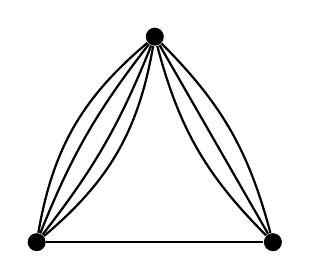
\begin{tikzpicture}
            [scale=3.0,auto=center,every node/.style={circle, fill=black, inner sep=2.3pt}]
            \tikzstyle{edges} = [black, thick];

            \node (a1) at (-0.5,0.86) {};
            \node (a3) at (0,1.73)  {};
            \node (a2) at (0.5,0.86)  {};

            \draw[edges] (a1) -- (a2) ;
            \draw[edges] (a3) edge[bend right=20] (a1) ;
            \draw[edges] (a3) edge[bend right=-20] (a1);
            \draw[edges] (a3) edge[bend right=8] (a1) ;
            \draw[edges] (a3) edge[bend right=-8] (a1);
            \draw[edges] (a3) edge[bend right=15] (a2);
            \draw[edges] (a3) edge[bend right=-15] (a2);
            \draw[edges] (a3) -- (a2);
        \end{tikzpicture}
        \caption{The edges of the left are labelled by $\{1,5,6,8\}$, the edges on the right by $\{3,4,7\}$ and the bottom one by $\{2\}$.}\label{fig:graph}
    \end{figure}
\end{example}


Since the class of elementary split matroids contains all copaving matroids, and since the inverse Kazhdan--Lusztig polynomial is a valuative invariant, we may apply \cite[Theorem~1.4]{ferroni-schroter} to compute $Q_{\M}(x)$ for any corank $2$ matroid without coloops.

\begin{theorem}
    Let $\M$ be a corank $2$ matroid without coloops. Assume that for each $r$, $\lambda_r$ denotes the number of stressed subsets of rank $r$ and size $r+1$ in $\M$. Then
    \begin{align*}
        Q_{\M}(x) & = Q_{\U_{n-2,n}}(x) - \sum_{r} \lambda_{r} \sum_{a=2}^{n-r-1} \left(Q_{\C_{a,n+1-a}}(x) - Q_{\U_{a-1,a}}(x)\, Q_{\U_{n-a-1,n-a}}(x)\right), \\
        Y_{\M}(x) & = Y_{\U_{n-2,n}}(x) - \sum_{r} \lambda_{r} \sum_{a=2}^{n-r-1} \left(Y_{\C_{a,n+1-a}}(x) - Y_{\U_{a-1,a}}(x)\, Y_{\U_{n-a-1,n-a}}(x)\right).
    \end{align*}
    In particular, if $\M$ arises from a partition $\lambda$ of $[n]$, then
    \begin{align*}
        Q_{\M}(x) & = Q_{\U_{n-2,n}}(x) - \sum_{\substack{S\in \lambda \\ |S|\geq 2}} \sum_{a=2}^{|S|} \left(Q_{\C_{a,n+1-a}}(x) - Q_{\U_{a-1,a}}(x)\, Q_{\U_{n-a-1,n-a}}(x)\right),\\
        Y_{\M}(x) & = Y_{\U_{n-2,n}}(x) - \sum_{\substack{S\in \lambda \\ |S|\geq 2}}\sum_{a=2}^{|S|} \left(Y_{\C_{a,n+1-a}}(x) - Y_{\U_{a-1,a}}(x)\, Y_{\U_{n-a-1,n-a}}(x)\right).
    \end{align*}
\end{theorem}

\begin{proof}
    By a direct application of \cite[Theorem~5.3]{ferroni-schroter}, we obtain that for any coloopless corank $2$ matroid on $n$ elements, the following equality holds:
    \[ Q_{\M}(x) = Q_{\U_{n-2,n}}(x) - \sum_{r,h} \lambda_{r,h} \left( Q_{\LL_{r,n-2,h,n}}(x) - Q_{\U_{n-2-r,n-h}}(x) Q_{\U_{r,h}}(x)\right),\]
    where $\lambda_{r,h}$ is the number of stressed subsets of $\M$ that have rank $r$ and size $h$. Since $\M$ has corank $2$, the definition of being a stressed subset implies that $h\in \{r,r+1,r+2\}$, and in fact the cases $h=r$ and $h=r+2$ cannot happen. Thus,
    \[ Q_{\M}(x) = Q_{\U_{n-2,n}}(x) - \sum_{h} \lambda_{r} \left( Q_{\LL_{r,n-2,r+1,n}}(x) - Q_{\U_{n-r-2,n-r-1}}(x) Q_{\U_{r,r+1}}(x)\right),\]
    where now $\lambda_r$ counts the number of stressed subsets of rank $r$ and size $r+1$. By \cite[Corollary~5.7]{ferroni-schroter}, since the inverse Kazhdan--Lusztig polynomial is a valuative invariant, we obtain:
    \[ Q_{\LL_{r,n-2,r+1,n}}(x) = \sum_{a=2}^{n-r-1} Q_{\C_{a,n+1-a}}(x) - \sum_{a=2}^{n-r-2} Q_{\U_{a-1,a}}(x)\, Q_{\U_{n-a-1,n-a}}(x),\]
    which yields:
    \[ Q_{\LL_{r,n-2,r+1,n}}(x)- Q_{\U_{n-r-2,n-r-1}}(x) Q_{\U_{r,r+1}}(x) = \sum_{a=2}^{n-r-1} \left(Q_{\C_{a,n+1-a}}(x) - Q_{\U_{a-1,a}}(x)\, Q_{\U_{n-a-1,n-a}}(x)\right).\]
    Putting all the pieces together, we obtain:
    \[ Q_{\M}(x) = Q_{\U_{n-2,n}}(x) - \sum_{h} \lambda_{r} \sum_{a=2}^{n-r-1} \left(Q_{\C_{a,n+1-a}}(x) - Q_{\U_{a-1,a}}(x)\, Q_{\U_{n-a-1,n-a}}(x)\right),\]
    as desired.
\end{proof}

\begin{theorem}
    The matroid induced by partitioning the set $\{1,\ldots,21\}$ into six parts of sizes $(4,4,4,3,3,3)$ is a counterexample to the real-rootedness conjecture of Xie--Zhang.
\end{theorem}

\begin{proof}
    Computing the inverse Kazhdan--Lusztig polynomial via the preceding theorem results in:
    \begin{multline*} Q_{\M}(x) = 71162 \, x^{9} + 232662 \, x^{8} + 350404 \, x^{7} + 323646 \, x^{6}\\ + 215169 \, x^{5} + 106659 \, x^{4} + 39217 \, x^{3} + 10323 \, x^{2} + 1790 \, x + 163.
    \end{multline*}
    After taking the Hadamard product with $(1+x)^9$, we obtain:
    \begin{multline*}(1+x)^9 * Q_{\M}(x)= 71162 \, x^{9} + 2093958 \, x^{8} + 12614544 \, x^{7} + 27186264 \, x^{6}\\ + 27111294 \, x^{5} + 13439034 \, x^{4} + 3294228 \, x^{3} + 371628 \, x^{2} + 16110 \, x + 163.
    \end{multline*}
    According to SageMath, this polynomial is not real-rooted. It possesses two complex conjugate zeros near $-1.0297\pm 0.1097\,i$.
\end{proof}


Since $Q_{\C_{a,n+1-a}}(x)$ can be computed in terms of inverse KL polynomials of uniform matroids via the deletion formula, this gives a closed formula for any corank $2$ matroid.




\bibliographystyle{amsalpha}
\bibliography{references}

\end{document}